%!TEX root=../GaugeCNNTheory.tex


\subsection{Isometry equivariance of kernel field transforms and \textit{GM}-convolutions}
\label{sec:isometry_equivariance}


We now turn to investigate under which conditions kernel field transforms and $\GM$-convolutions are equivariant w.r.t. the action of isometries on feature fields.
As the action on the $G$-associated feature vector bundles is only defined for $G$-structure preserving isometries, we will formulate all statements for the subgroup $\IsomGM \leq \IsomM$ or subgroups $\I \leq \IsomGM$ thereof.
One can of course always consider structure groups $G\geq\O{d}$, for which $\IsomGM = \IsomM$.


The equivariance of a kernel field transform, and thus $\GM$-convolutions, is defined as follows:
\begin{dfn}[Isometry equivariant kernel field transform]
\label{dfn:isometry_equivariance}
    Let ${\TK: \Gamma(\Ain) \to \Gamma(\Aout)}$ be a kernel field transform.
    Then $\TK$ is said to be \emph{equivariant w.r.t the action of isometries} in a subgroup $\I \leq \IsomGM$ if it commutes with this action, that is, if the following property holds:
    \begin{align}\label{eq:isom_equivariance_kernel_field_trafo_def}
        \TK \big( \phi\rhd\!f \big) \ =\ \phi\rhd\! \big( \TK(f) \big)
        \qquad \forall\ \ f\in\Gamma(\Ain), \ \ \phi\in \I
    \end{align}
    In terms of a diagram, $\TK$ is equivariant w.r.t isometries in $\I$ if
    \begin{equation}
    \begin{tikzcd}[column sep=70pt, row sep=35, font=\normalsize]
        \Gamma(\Ain)
            \arrow[r, "\TK"]
            \arrow[d, "\phi\,\rhd"']
        &
        \Gamma(\Aout)
            \arrow[d, "\phi\,\rhd"]
        \\
        \Gamma(\Ain)
            \arrow[r, "\TK"']
        &
        \Gamma(\Aout)
    \end{tikzcd}
    \end{equation}
    commutes for all $\phi \in \I$.
\end{dfn}
A visualization of this definition is given in Fig.~\ref{fig:lizard_conv_egg}.
In the following Section~\ref{sec:isometry_constraint} we will derive a constraint on kernel fields in order for the corresponding kernel field transform to be isometry equivariant.
The geometrically intuitive result which we obtain is that the kernel field itself is required to be invariant under the action of isometries, which implies a form of weight sharing over the isometry orbits; see Fig.~\ref{fig:isom_invariant_kernel_field_multiple_orbits}.
Section~\ref{sec:isom_equiv_GM_conv} applies these insights to the more specific case of $\GM$-convolutions and $\GM$-convolutional kernel fields.
It turns out that $\GM$-convolutions are by the $G$-steerability of their template kernel automatically equivariant with respect to \emph{any} isometry in $\IsomGM$.








\subsubsection{Isometry equivariance of general kernel field transforms}
\label{sec:isometry_constraint}

The main result of this section, Theorem~\ref{thm:isometry_equivariant_kernel_field_trafos}, states that \emph{a kernel field transform $\TK$ is isometry equivariant if and only if its underlying kernel field $\K$ is invariant under isometries}.
To make sense of this statement we start by defining the transformation behavior of kernel fields when being acted on by isometries.
\begin{dfn}[Isometry action on kernel fields]
\label{dfn:isometry_action_kernel_fields}
    Let $\K: \TM \to \Hom(\Ain,\Aout)$ be a kernel field.
    An isometry $\phi \in \IsomGM$ acts on $\K$ via the kernel field pushforward
    \begin{align}\label{eq:kernel_constraint_isom_full_1}
        \dphiK \K\ :=\ \dphiHom \!\circ \K \circ \dphiTMinv \,.
    \end{align}
    Intuitively, this pushforward of kernel fields can be thought of as moving the individual kernels $\Kp$ at points $p\in M$ along the orbits of the isometry group to $\phi(p)$.
\end{dfn}
Since kernel fields are defined to be bundle $M$-morphisms, that is, to satisfy $\piHom \K = \piTM$, their pushforward is only well defined if it preserves this property.
This is guaranteed since the pushforward on the tangent bundle and homomorphism bundle are bundle maps, satisfying $\piTM \circ \dphiTM = \phi \circ \piTM$ (Eq.~\eqref{cd:pushforward_TM}) and ${\piHom \circ \dphiHom = \phi \circ \piHom}$ (Eq.~\eqref{cd:associated_bdl_automorphism}), respectively:
\begin{align}
    \piHom\, \dphiK \K
    \ &=\ \piHom\, \dphiHom \K\; \dphiTMinv \notag \\
    \ &=\ \phi\, \piHom\, \K\; \dphiTMinv \notag \\
    \ &=\ \phi\, \piTM\, \dphiTMinv \notag \\
    \ &=\ \phi\, \phiinv\, \piTM \notag \\
    \ &=\ \piTM
\end{align}
We visualize the definition of the isometry action on kernel fields by a commutative diagram:
\begin{equation}
    \begin{tikzcd}[row sep=3.5em, column sep=2.8em]
        % ROW 1
        &[3.5ex] M & \\
        % ROW 2
        \TM  \arrow[ru, "\piTM"]
            \arrow[rr, pos=.56, "\dphiK \K"']
        & &
        \mkern-3mu
        \Hom(\Ain,\Aout)
            \arrow[lu, "\piHom"']
        \\
        % ROW 3
        \TM  \arrow[rd, "\piTM"']
            \arrow[rr, pos=.57, "\K"]
            \arrow[u, "\dphiTM"]
        & &
        \mkern-3mu
        \Hom(\Ain,\Aout)
            \arrow[ld, "\piHom"]
            \arrow[u, "\dphiHom"']
        \\
        % ROW 4
        & M 
            \arrow[uuu, rounded corners, to path={ 
                    -- ([xshift=-25ex]\tikztostart.west) 
                    --node[left, pos=.515]{\small$\phi$} ([xshift=-25ex]\tikztotarget.west) 
                    -- (\tikztotarget.west)
                    }]
        &
    \end{tikzcd}
    \quad
\end{equation}
The bottom part of this diagram shows the coordinate free kernel field $\K$ from the diagram in Eq.~\eqref{eq:kernel_bundle_map} while the upper part shows its pushforward $\dphiK \K = \dphiHom \!\circ \K \circ \dphiTMinv$ by $\phi \in \IsomGM$.
The commutativity of the leftmost arrow, which asserts that $\dphiK$ moves kernels from $p$ to $\phi(p)$, follows from $\dphiTM$ and $\dphiHom$ both being bundle maps over $\phi$.


We proceed by defining isometry invariant kernels fields -- a visualization is found in Fig.~\ref{fig:isom_invariant_kernel_field_multiple_orbits}.
\begin{dfn}[Isometry invariant kernel fields]
\label{dfn:isometry_invariant_kernel_fields}
    A kernel field $\K$ is said to be \emph{invariant%
    \footnote{
        Instead of saying that $\K$ is \emph{invariant}, one could call it \emph{equivariant} since it satisfies
        $\dphiHom \!\circ \K \,=\ \K \circ \dphiTM \ \forall \phi\in\I$.
        In general, any function which is equivariant w.r.t. certain group actions on its domain and codomain is \emph{itself} invariant under pre- and postcomposition with the actions on its domain and codomain as in Eq.~\eqref{eq:kernel_constraint_isom_full_1}.
    }
    under isometries} in $\I \leq \IsomGM$ if it satisfies the constraint $\dphiK \K = \K$ for all $\phi \in \I$.
    We denote the space of isometry invariant kernel fields by
    \begin{align}\label{eq:KIfull_def}
        \KIfull :=
            \pig\{\mkern2mu \K\mkern-2mu:\TM\to \Hom(\Ain,\Aout) \ \ \textup{smooth}\ \,\pig|\; 
            \piHom\!\circ\K = \piTM \,,\ \ \ 
            \dphiK \K  = \K \quad \forall \phi\in\I \,\pig\} \,.
    \end{align}
\end{dfn}
By writing out $\dphiK$, the invariance constraint reads
\begin{align}\label{eq:kernel_constraint_isom_full_1}
    \dphiHom \!\circ \K \circ \dphiTMinv \,=\ \K \qquad \forall \phi\in\I \,,
\end{align}
which, after further expanding $\dphiHom$ as defined in Eq.~\eqref{eq:pushforward_Hom_def}, becomes:
\begin{align}\label{eq:kernel_constraint_isom_full_2}
    \dphiAout
    \K \big(\dphiTMinv v\big) \ 
    \dphiAininv
    =\,
    \K(v) \qquad \forall\ v\in \TM,\ \ \forall \phi \in \I
\end{align}
Note the similarity of these kernel field constraints in
Eqs.~\eqref{eq:kernel_constraint_isom_full_1} and~\eqref{eq:kernel_constraint_isom_full_2} with the $G$-steerability constraint on template kernels in Eqs.~\eqref{eq:G_steerable_space_in_dfn_Hom} and~\eqref{eq:G_steerable_space_in_dfn_classical}, respectively.
Indeed, both constraints are closely related and imply each other to a certain extent as we will show in the following Section~\ref{sec:isom_equiv_GM_conv} on isometry equivariant $\GM$-convolutions.


\begin{SCfigure}
    \centering
    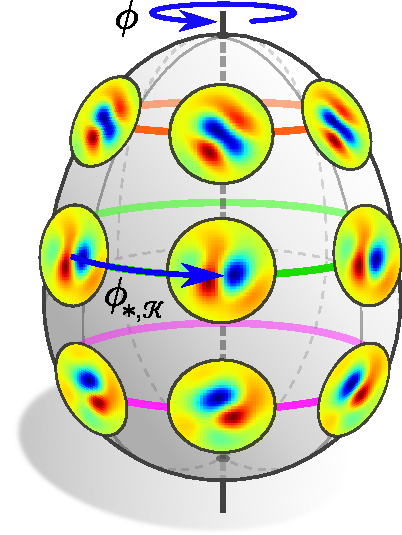
\includegraphics[width=.28\textwidth]{figures/isometry_egg_invariant_kernel.pdf}
    \hspace{10ex}
    \captionsetup{width=1.2\textwidth}
    \caption[]{\small
        Visualization of an invariant kernel field $\K$ for the case of an isometry (sub)group $\I = \SO2$.
        The invariance constraint requires $\dphiK \K := \dphiHom \K \dphiTMinv = \K$ for any $\phi$ in $\I$.
        It enforces kernels to be shared over the orbits $\I.p := \{\phi(p) \,|\, \phi \in \I\}$ of the action but allows for different kernels on different orbits.
        Theorem~\ref{thm:isometry_equivariant_kernel_field_trafos} proves that invariant kernel fields and equivariant kernel field transforms imply each other.
        This is intuitively clear since a specific pattern in the feature field at~$p\in M$ will evoke the same response when being transported to $\phi(p)$ if and only if the kernels at both points coincide.
        For the choice of $\I = \O2$ as isometry group, the kernels would additionally have to satisfy a reflectional constraint; see Fig.~\ref{fig:isom_invariant_kernel_field_quotient}.
        \\\protect\rule{0ex}{2.ex}
        }
    \label{fig:isom_invariant_kernel_field_multiple_orbits}
\end{SCfigure}


The following theorem proves that kernel fields which are invariant under isometries do indeed correspond to isometry equivariant kernel field transforms:
\begin{thm}[Equivariant kernel field transform $\Leftrightarrow$ invariant kernel field]
\label{thm:isometry_equivariant_kernel_field_trafos}
    \ A kernel field transform $\TK: \Gamma(\Ain)\to \Gamma(\Aout)$ is equivariant w.r.t. isometries in $\I \leq \IsomGM$ according to Def.~\ref{dfn:isometry_equivariance} if and only if
    the underlying kernel field~$\K$ is invariant under isometries according to Def.~\ref{dfn:isometry_invariant_kernel_fields}, that is,
    \begin{align}
        \TK(\phi \rhd f) \,=\, \phi \rhd \TK(f)
        \quad\forall\; \phi \in \I\,,\ f\in\Gamma(\Ain)
        \quad \Longleftrightarrow \quad
        \dphiK \K = \K
        \quad\forall\, \phi \in \I
    \end{align}
\end{thm}
\begin{proof}
    To prove this theorem, we write out the kernel field transforms and feature field pushforwards on both sides of the isometry equivariance condition in Eq.~\eqref{eq:isom_equivariance_kernel_field_trafo_def}.
    The statement follows from a comparison of both sides after a few algebraic manipulations.

    We start with the right-hand side of Eq.~\eqref{eq:isom_equivariance_kernel_field_trafo_def}:
    \begin{align}
        \big[ \phi \rhd \TK(f) \big](p)
        \ &\overset{(1)}{=}\ \ 
            \dphiAout \big[ \TK(f) \big] \big( \phi^{-1}(p) \big) \notag \\[1ex]
        \ &\overset{(2)}{=}\ \ 
            \dphiAout \mkern-8mu
            \int\limits_{T_{\!\phiinv\mkern-1mu(p)}\mkern-2muM}\!\!
            \mkern-6mu \K(v) \ 
            \big[\mkern-2mu \Expsphiinvpf \mkern1mu\big] (v)
            \,\ dv \notag \\
        \ &\overset{(3)}{=}\ \ 
            \dphiAout \mkern-8mu
            \int\limits_{T_{\!\phiinv\mkern-1mu(p)}\mkern-2muM}\!\!
            \mkern-6mu \K(v) \ 
            \dphiAin^{-1} \big[\mkern-2mu \Expsp\! \big(\phi \rhd f\big) \mkern1mu\big] \big( \dphiTM (v) \big)
            \,\ dv \notag \\
        \ &\overset{(4)}{=}\ \ 
            \int\limits_{\TpM}
            \dphiAout
            \K\big( \dphiTM^{-1} \tilde{v} \big) \ 
            \dphiAin^{-1} \big[\mkern-2mu \Expsp\! \big(\phi \rhd f\big) \mkern1mu\big] (\tilde{v})
            \,\ d\tilde{v} \notag \\
        \ &\overset{(5)}{=}\ \ 
            \int\limits_{\TpM}
            \big[ \dphiHom \K\, \dphiTM^{-1} \big] (\tilde{v}) \ 
            \big[\mkern-2mu \Expsp\! \big(\phi \rhd f\big) \mkern1mu\big] (\tilde{v})
            \,\ d\tilde{v} \notag \\
        \ &\overset{(6)}{=}\ \ 
            \int\limits_{\TpM}
            \big[ \dphiK \K \big] (\tilde{v}) \ 
            \big[\mkern-2mu \Expsp\! \big(\phi \rhd f\big) \mkern1mu\big] (\tilde{v})
            \,\ d\tilde{v}
    \end{align}
    Steps~$(1)$ and~$(2)$ expand the isometry action $\rhd$ on feature fields (Def.\ref{dfn:isometry_pushforward}) and the kernel field transform (Def.~\ref{dfn:kernel_field_trafo}).
    The transformation law of the field's transporter pullback in Theorem~\ref{thm:transporter_pullback_isometry_action}, which relies on the $\IsomGM$-invariance of the $G$-compatible connection, justifies step~$(3)$.
    Step~$(4)$ substitutes $v$ with $\tilde{v} = \dphiTM v$.
    Since $\phi$ is an isometry, the change of volume equates to~$1$.
    Steps~$(5)$ and~$(6)$ identify the action of the kernel pushforward~$\dphiK$, Def.~\ref{dfn:isometry_action_kernel_fields}.
    The resulting statement is quite intuitive:
    A transformation of the kernel field transform's output corresponds to a simultaneous transformation of its input \emph{and} kernel field.

    Writing out the left-hand side yields
    \begin{align}
        \big[ \TK \big(\phi \rhd f\big) \big](p)
        \ =\ \int\limits_{\TpM}
                \K(v) \ 
                \big[\mkern-2mu \Expsp\!\big( \phi\rhd f\big) \mkern1mu\big] (v)
                \,\ dv \,,
    \end{align}
    which is equivalent to the right-hand side \emph{up to} the transformation of the kernel field.

    Isometry equivariance requires both expressions to agree for arbitrary fields $f\in\Gamma(\Ain)$, points $p\in M$ and isometries $\phi\in\I$.
    This is the case if and only if $\dphiK \K = \K$ holds for any $\phi \in \I$, i.e. if the kernel field is invariant under the action of isometries.
\end{proof}
Note that this proof would have been very cumbersome to work out in (a $G$-atlas of) local trivializations.
The global, coordinate free description of kernel field transforms allows for a simple proof without having to worry that the isometries move features between different local trivializations.


At this point we could proceed with a further investigation of isometry invariant kernel fields:
since the invariance constraint implies kernels to be shared over orbits of the isometry group, a description of the entire kernel field on the full manifold is redundant.
It is therefore possible to reduce the description of such kernel fields to kernel fields on quotient spaces.
As this analysis is not required to prove the isometry equivariance of $\GM$-convolutions and requires some technical definitions, we postpone it to Section~\ref{sec:quotient_kernel_fields}




















\subsubsection{Isometry equivariance of \textit{GM}-convolutions}
\label{sec:isom_equiv_GM_conv}

Recall that $\GM$-convolutions (Def.~\ref{dfn:coord_free_conv}) were defined as specific kernel field transforms with $\GM$-convolutional kernel fields (Def.~\ref{dfn:conv_kernel_field}).
The results on the isometry equivariance of kernel field transforms therefore immediately apply to $\GM$-convolutions as well.
However, in addition to the isometry invariance constraint in Eq.~\eqref{eq:kernel_constraint_isom_full_1}, $\GM$-convolutional kernel fields need to satisfy the $G$-steerability constraint on the template kernel from Eq.~\eqref{eq:G_steerable_space_in_dfn_Hom} and share weights over the $G$-structure according to Eq.~\eqref{eq:conv_kernel_field_def_ptwise}.
In order for the $\GM$-convolution to be isometry equivariant, all of these constraints have to be satisfied simultaneously.
Intuitively, this implies that the convolutional weight sharing needs to agree with the isometry induced weight sharing over orbits.
Luckily it turns out that this is automatically the case for the isometries under consideration:
$\GM$-convolutions share weights over the $G$-structure and the isometries in $\IsomGM$ preserve the $G$-structure such that \emph{$\GM$-convolutional kernel fields are guaranteed to be $\IsomGM$ invariant}.
In coordinates, this reflects in the $\IsomGM$-induced gauge transformations $g_\phi^{A\widetilde{A}}(p)$ taking values in the structure group $G$, such that they are explained away by the $G$-steerability of the template kernels.


To make these arguments more rigorous, consider a $\GM$-convolution $K\star: \Gamma(\Ain) \to \Gamma(\Aout)$ with some $G$-steerable kernel $K \in \KG$, which is by Def.~\ref{dfn:coord_free_conv} just the kernel field transform $\TKK$ with the $\GM$-convolutional kernel field $\KK$.
By Theorem~\ref{thm:isometry_equivariant_kernel_field_trafos}, the $\GM$-convolution is therefore exactly then $\IsomGM$-equivariant if~$\KK$ is $\IsomGM$-invariant, i.e. when it satisfies $\dphiK \KK = \dphiHom \circ \KK \circ \dphiTMinv = \KK$ for any $\phi \in \IsomGM$.
This constraint on the full kernel field is equivalently expressed by a set of constraints on the individual convolution kernels that make up the field:
\begin{align}\label{eq:KK_constraint_ptwise_abstract}
    \dphiHom \circ \KKp \circ \dphiTMinv \ &=\ \KKphip \qquad \forall\ p\in M,\ \ \phi \in \IsomGM
\end{align}
Considering a specific point $p\in M$, we choose arbitrary gauges $\widetilde{A}$ at $p$ and $A$ at $\phi(p)$ from the $G$-atlas.
The $\GM$-convolutional kernel field is by Def.~\ref{dfn:conv_kernel_field} at $p$ and $\phi(p)$ given by
\begin{align}
    \KKp    := \big(\psiHomp^{\widetilde{A}} \big)^{-1} \circ \frac{K}{\sqrt{|\eta_p^{\widetilde{A}}|}} \circ \psiTMp^{\widetilde{A}}
    \qquad \textup{and} \qquad
    \KKphip := \big(\psiHomphip^A            \big)^{-1} \circ \frac{K}{\sqrt{|\eta_{\phi(p)}^A|}}       \circ \psiTMphip^A \,.
\end{align}
Plugging these expressions into the constraint in Eq.~\eqref{eq:KK_constraint_ptwise_abstract} for the fixed $p$ and identifying $\dphiHom \big(\psiHomp^{\widetilde{A}} \big)^{-1}$ with $\big( \psiHomp^{\widetilde{A}}\, \dphiHom^{-1}  \big)^{-1}$ yields:
\begin{align}\label{eq:GM-conv_kernel_field_isom_invariance_1}
    \big( \psiHomp^{\widetilde{A}}\, \dphiHom^{-1}  \big)^{-1} \circ \frac{K}{\sqrt{|\eta_p^{\widetilde{A}}|}} \circ \psiTMp^{\widetilde{A}}\, \dphiTMinv
    \,\ &=\,\ \big(\psiHomphip^A \big)^{-1} \circ \frac{K}{\sqrt{|\eta_{\phi(p)}^A|}} \circ \psiTMphip^A
    \qquad \forall\ \phi \in \IsomGM
\end{align}
The isometry equivariance will therefore hold if the weight sharing via the isometry induced gauges $\psidotp^{\widetilde{A}} \dphidot$ agrees with the weight sharing via the original gauges $\psidotphip^A$ from $\phi(p)$.
Recall that the isometry induced gauges are by Theorem~\ref{thm:isom_GM_in_coords} for isometries in $\IsomGM$ guaranteed to be compatible with the $G$-atlases (of the corresponding bundle).
As shown in Eq.~\eqref{eq:arbitrariness_gauge_GM_kernel_field_def}, the particular choice of gauge, relative to which the $G$-steerable template kernel is oriented, is irrelevant, as long as the gauges are $G$-compatible.
Since all derivations were independent from the chosen point $p$ and the particular choice of gauges, this implies that $\GM$-convolutions are by design guaranteed to be $\IsomGM$-equivariant.


To gain a better intuition for this result it is worth to make the induced, $G$-valued gauge transformations $g_\phi^{A\widetilde{A}}(p)$ explicit.
To this end, note that the commutativity of the diagrams in Eqs.~\eqref{cd:pushforward_A_coord} and~\eqref{cd:pushforward_TM_coord} implies
$\psiHomp^{\widetilde{A}}\, \dphiHominv = \rhoHom\big( g_\phi^{A\widetilde{A}}(p) \big)^{-1} \psiHomphip^A$ and
$\psiTMp^{\widetilde{A}}\,  \dphiTMinv  =        \big( g_\phi^{A\widetilde{A}}(p) \big)^{-1} \psiTMphip^A$.
Inserting these coordinate expressions into the constraint in Eq.~\eqref{eq:GM-conv_kernel_field_isom_invariance_1} leads to the requirement that
\begin{align}\label{eq:GM-conv_kernel_field_isom_invariance_2}
    \Big(\mkern-1.5mu \rhoHom\big( g_\phi^{A\widetilde{A}}(p) \big)^{-1} \psiHomphip^A \mkern-1.5mu\Big)^{-1}
    \!\circ \frac{K}{\sqrt{|\eta_p^{\widetilde{A}}|}} \circ \big( g_\phi^{A\widetilde{A}}(p) \big)^{-1} \psiTMphip^A
    \ &=\ \big(\psiHomphip^A \big)^{-1} \!\circ \frac{K}{\sqrt{|\eta_{\phi(p)}^A|}} \circ \psiTMphip^A
\end{align}
needs to hold for any isometry $\phi$ in~$\IsomGM$.
By expanding the inverse on the left-hand side, using that
${\sqrt{|\eta_p^{\widetilde{A}}|} \,= \sqrt{|\eta_{\phi(p)}^A|} \cdot \big|\mkern-2mu \det g^{A\widetilde{A}}_\phi(p) \big|}$
and dropping the gauges, which is possible since they are isomorphisms, we end up with the constraint
\begin{align}\label{eq:GM_conv_isom_constraint_coords}
    \frac{1}{\big|\mkern-2mu \det g^{A\widetilde{A}}_\phi(p) \big|} \,
    \rhoHom\Big(g^{A\widetilde{A}}_\phi(p)\Big) \circ K \circ \Big(g^{A\widetilde{A}}_\phi(p)\Big)^{-1} \ =\ K
    \qquad \forall\ \phi \in \IsomGM \,,
\end{align}
which looks \emph{exactly} like the $G$-steerability kernel constraint on~$K$ from Def.~\ref{dfn:G-steerable_kernel_def_43}.
Recall that the isometry induced gauge transformations $g_\phi^{A\widetilde{A}}(p)$ are by Theorem~\ref{thm:isom_GM_in_coords} guaranteed to be $G$-valued if~$\phi$ is an element of $\IsomGM$.
The constraint in Eq.~\eqref{eq:GM_conv_isom_constraint_coords} is therefore always satisfied by the $G$-steerability of~$K$.

The derived results on the $\IsomGM$-invariance of $\GM$-convolutional kernel fields $\KK$ are concisely summarized by the statement that the following diagram is guaranteed to be commutative if $K$ is $G$-steerable and if $\phi \in \IsomGM$ is $G$-structure preserving:
\begin{equation}
    \begin{tikzcd}[row sep=4.em, column sep=5.5em] %,
        % ROW 1
        & &[-2.7em] U^A &[-2.7em] & \\[-1em]
        % ROW 2
        U^A \mkern-2mu\times\mkern-1mu \R^d
            \arrow[rrrr, rounded corners, to path={ 
                    -- ([yshift=15ex]\tikztostart.north) 
                    --node[above]{\small
                            $\id\times \pig( \rhoHom\big(g'^{A\widetilde{A}}_\phi\big) \circ K \big/\mkern-2mu \sqrt{|\eta^A|} \circ \big(g'^{A\widetilde{A}}_\phi\big)^{-1} \pig)$
                            } ([yshift=15ex]\tikztotarget.north) 
                    -- (\tikztotarget.north)
                    }]
        &
        \,\piTM^{-1}\big(U^A\big)
            \arrow[ru, "\piTM"]
            \arrow[rr, "\dphiK \KK"']
            \arrow[l, "\PsiTM^A"']
        & &
        \piHom^{-1}\big(U^A\big)
            \arrow[lu, "\piHom"']
            \arrow[r, "\PsiHom^A"]
        &
        U^A \mkern-2mu\times\mkern-1mu \R^{\cout\times\cin}
        \\
        % ROW 3
        U^{\widetilde{A}} \mkern-2mu\times\mkern-1mu \R^d
            \arrow[u, "\phi \times g_\phi^{A\widetilde{A}}\cdot"']
            \arrow[rrrr, rounded corners, to path={ 
                    -- ([yshift=-15ex]\tikztostart.south) 
                    --node[below]{\small$\id\times K \big/\mkern-2mu \sqrt{|\eta^{\widetilde{A}}|}$} ([yshift=-15ex]\tikztotarget.south) 
                    -- (\tikztotarget.south)
                    }]
        &
        \piTM^{-1}\big(U^{\widetilde{A}}\big)
            \arrow[rd, "\piTM"']
            \arrow[rr, "\KK"]
            \arrow[u, "\dphiTM"]
            \arrow[l, "\PsiTM^{\widetilde{A}}"]
        & &
        \piHom^{-1}\big(U^{\widetilde{A}}\big)
            \arrow[ld, "\piHom"]
            \arrow[u, "\dphiHom"']
            \arrow[r, "\PsiHom^{\widetilde{A}}"']
        &
        U^{\widetilde{A}} \mkern-2mu\times\mkern-1mu \R^{\cout\times\cin}
            \arrow[u, "\phi \times \rhoHom\big(g_\phi^{A\widetilde{A}}\big)"]
        \\[-1em]
        % ROW 4
        & & U^{\widetilde{A}}
        & &
    \end{tikzcd}
\end{equation}
Here we defined the pullback $g_\phi'^{A\widetilde{A}} := g_\phi^{A\widetilde{A}} \circ \phi^{-1} : U^A \to G$ of the isometry pushforward coordinatization from $U^{\widetilde{A}}$ to $U^A$ for notational convenience.


Together with Theorem~\ref{thm:isometry_equivariant_kernel_field_trafos}, the $\IsomGM$-invariance of $\GM$-convolutional kernel fields implies the $\IsomGM$-equivariance of $\GM$-convolutions:
\begin{thm}[Isometry equivariance of $\GM$-convolutions]
\label{thm:isom_equiv_GM_conv}
    A $\GM$-convolution $K\star: \Gamma(\Ain)\to \Gamma(\Aout)$ with a $G$-steerable kernel $K\in\KG$ is equivariant with respect to all $G$-structure preserving isometries $\phi \in \IsomGM$, that is,
    \begin{align}
        K \star \big( \phi \rhd f \big) \ =\ 
        \phi \rhd \big( K \star  f \big)
        \qquad \forall\ \ f\in\Gamma(\Ain), \ \ \phi\in \IsomGM \,.
    \end{align}
    The following diagram commutes therefore for every $\phi \in \IsomGM$:
    \begin{equation}
    \begin{tikzcd}[column sep=60pt, row sep=35, font=\normalsize]
        \Gamma(\Ain)
            \arrow[r, "K\star"]
            \arrow[d, "\phi\,\rhd\,"']
        &
        \Gamma(\Aout)
            \arrow[d, "\,\phi\,\rhd"]
        \\
        \Gamma(\Ain)
            \arrow[r, "K\star"']
        &
        \Gamma(\Aout)
    \end{tikzcd}
    \end{equation}
\end{thm}
\begin{proof}
    The proof was given in the discussion prior to the theorem.
\end{proof}



Having this general result on $\GM$-convolutions derived, we will now discuss some special cases for specific choices of structure groups~$G$.
Firstly, for orthogonal structure groups $G=\O{d}$ (or supergroups of it), the convolution will commute with \emph{any} isometry:
\begin{thm}[Full isometry equivariance of $\OM$-convolutions]
\label{thm:Od_equiv_OM_conv}
    $\OM$-convolutions are equivariant w.r.t. the action of \emph{any} isometry $\phi \in \IsomM$ on feature fields.
    More generally, any $\GM$-convolution for $G$-structures with structure groups $G\geq\O{d}$ is fully isometry equivariant.
\end{thm}
\begin{proof}
    The statement follows from Theorem~\eqref{thm:isom_equiv_GM_conv} by observing that $\IsomGM = \IsomM$ is guaranteed for structure groups $G \geq \O{d}$.
    The latter was discussed in Eq.~\eqref{eq:isomM_isomOM}.
\end{proof}
This result relies essentially on the fact that isometries are defined as that subgroup of diffeomorphisms on~$M$ which induce $\O{d}$-structure automorphisms.
Less abstractly stated, $\IsomM$ is by definition that subgroup of diffeomorphisms which respect the Riemannian metric~$\eta$ of~$M$ and the corresponding $\O{d}$-structure $\OM$ is equivalent information to the metric.


On orientable Riemannian manifolds one can furthermore pick an orientation (frame handedness), which together with the metric defines an $\SO{d}$-structure $\SOM$.
The corresponding isometries which lift to $\SO{d}$ structure automorphisms are the orientation preserving isometries in $\IsomplusM$.
\begin{thm}[$\IsomplusM$ equivariance of $\SOM$-convolutions]
\label{thm:SOd_equiv_SOM_conv}
    $\SOM$-convolutions are equivariant w.r.t. the action of orientation preserving isometries $\phi \in \IsomplusM$ on feature fields.
\end{thm}
\begin{proof}
    This result follows from Theorem~\eqref{thm:isom_equiv_GM_conv} by observing that $\IsomSOM = \IsomplusM$.
\end{proof}
For instance, an $\SOM$-convolution for $M=\R^2$, corresponding to Fig~\ref{fig:SO2_structure_SE2}, is equivariant w.r.t. the action of the special Euclidean group $\Isom_+(\R^2) = \SE2$.
Similarly, an $\SOM$-convolution for $M=S^2$, corresponding to Fig~\ref{fig:SO2_structure_SO3}, is rotation equivariant with $\Isom_+(S^2) = \SO3$.


Note that the results of Theorems~\ref{thm:Od_equiv_OM_conv} and~\ref{thm:SOd_equiv_SOM_conv} depend only on the structure group $G$ but not on the particular choice of $G$-structure.
For subgroups $G$ of $\O{d}$ (or $\SO{d}$) things become more complicated.
In these cases the subgroups $\IsomGM$ of $\IsomM$ depend on the specific embedding of the $G$-structure~$\GM$ into~$\FM$.
This was for $G=\{e\}$ visualized in Fig.~\ref{fig:frame_field_automorphism}.
Specifically, Fig.~\ref{fig:frame_field_automorphism_1} shows the canonical $\{e\}$-structure of $\R^2$, which is fully translation equivariant, that is, $\IsomeM = \Trans_2 := (\R^2,+)$.
In contrast, Fig.~\ref{fig:frame_field_automorphism_2} shows an $\{e\}$-structure of $\R^2$ which is only translation equivariant along one axis such that $\IsomeM \cong \Trans_1 := (\R,+)$.
From the viewpoint of convolutional networks this result is very intuitive:
The $\{e\}$-steerable kernels in these examples are unconstrained, i.e. conventional convolution kernels.
They do therefore in general not carry any information about their responses when being applied relative to gauge transformed reference frames.
Since the frames, and therefore kernels, in Fig.~\ref{fig:frame_field_automorphism_2} are differently rotated along the ``left-right'' direction, the kernel responses change unpredictably when translating a signal in that direction.
If the template kernels would, however be $\SO2$-steerable, they could account for the rotation of frames.
This case corresponds to the situation in Fig~\ref{fig:SO2_structure_SE2}, i.e. an $\SOM$-convolution.
